\chapter{Inductancia}
\section{Inductancia mutua}

\begin{figure}[h]
\centering
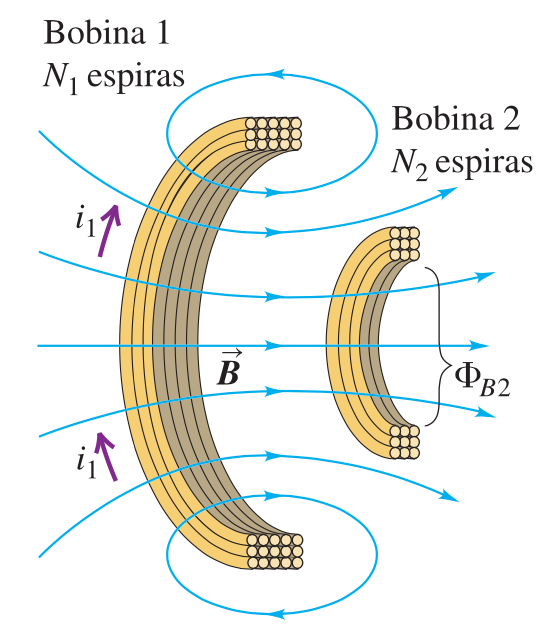
\includegraphics[scale=0.3]{fig/bobinas}
\caption{\textbf{Inductancia mutua}, si la corriente en la bobina 1 está cambiando, el flujo cambiante a través de la bobina 2 indice una fem en esta última}
\label{fig:bobinas}
\end{figure}
Interacción magnética entre dos alambres que trasnportan corrientes \textit{estables}; la corriente de uno de los alambres genera un campo magnético que ejerce una fuerza sobre la corriente entre el otro alambre. Cuando hay una corriente \textit{variable} en uno de los circuitos, surge una interacción adicional. Consideremos la situación de la figura
\ref{fig:bobinas}

Una corriente que circula por la bobina 1 produce un campo magnético $\vec{B}$ y, por lo tanto, un flujo magnético a través de la bobina 2. Si la corriente en la bobina 1 cambia, el flujo a través de la bobina 2 también cambia; de acuerdo con la ley de Faraday, esto induce una fem en la bobina 2. De este modo, un cambio en la corriente de un circuito puede inducir otra corriente en un segundo circuito.
Una corriente $i_1$\footnote{Denotamos con $i$ a una corriente variable en el tiempo } establece un campo magnético (indicado por las líneas de color azul), y algunas de estas líneas de campo pasan a través de la bobina 2. Denotaremos con $\Phi_{B2}$ el flujo magnético a través de \textit{cada} espira de la bobina 2, causado por la corriente $i_1$ en la bobina 1. (Si el flujo es diferente a través de las distintas espiras de la bobina, entonces $\Phi_{B2}$ denota el flujo  \textit{medio}). El campo magnético es proporcional a $i_1$, de manera que $\Phi_{B2}$ también es proporcional a $i_1$. \textbf{Cuando $i_1$ cambia, $\Phi_{B2}$ cambia; este flujo cambiante induce una fem $\varepsilon_2$ en la bobina 2}, dada por
\begin{equation}\label{fem}
\varepsilon_2=-N_2\frac{d\Phi_{B2}}{dt}
\end{equation}
Podríamos representar la proporcionalidad entre $\Phi_{B2}$ e $i_1$ en la forma $\Phi_{B2}$ = (constante) $i_1$, pero, en vez de ello, es más conveniente incluir el número de espiras $N_2$ en la relación. Al introducir una constante de proporcionalidad $M_{21}$, llamada \textbf{inductancia mutua} de las dos bobinas, escribimos
\begin{equation}\label{30.2}
N_2\Phi_{B2}=M_{21}i_1
\end{equation}
donde $\Phi_{B2}$ es el flujo a través de una sola espira de la bobina 2. De ahí que,
\begin{equation}
N_2\frac{d\Phi_{B2}}{dt}=M_{21}\frac{di_1}{dt}
\end{equation}
y (\ref{fem}) se rescribe como
\begin{equation}
\varepsilon_2=-M_2\frac{di_1}{dt}
\end{equation}
Es decir, un cambio en la corriente $i_1$ en la bobina 1 induce una fem en la bobina 2, que es directamente proporcional a la tasa de cambio de $i_1$.

También se podría escribir la definición de la inductancia mutua, (\ref{30.2}), como
\begin{equation}
M_{21}=\frac{N_2\Phi_{B2}}{i_1}
\end{equation}
\textbf{Si las bobinas están en el vacío}, el flujo $\Phi_{B2}$ a través de cada espira de la bobina 2 es directamente proporcional a la corriente $i_1$. Entonces, la inductancia mutua $M_{21}$ es una constante que sólo depende de la geometría de las dos bobinas.
Podría volverse a hacer el análisis para el caso opuesto, en el que una corriente cambiante $i_2$ en la bobina 2 causa un flujo cambiante $\Phi_{B}2$ y una fem $\varepsilon_1$ en la bobina 1. Se encuentra que, \textbf{$M_{12}$ siempre es igual a $M_{21}$, aun cuando las dos bobinas no sean simétricas}. A este valor común $M$ lo llamamos simplemente \textbf{inductancia mutua}. Por tanto, tenemos:
\begin{equation}\marginnote{Fem mutuamente inducidas}
\boxed{\varepsilon_2=-M\frac{di_1}{dt}\quad\mathrm{y}\quad \varepsilon_1=-M\frac{di_2}{dt}\quad}
\end{equation}
donde la inductancia mutua $M$ es
\begin{equation}\marginnote{Inductancia mutua}
\boxed{M=\frac{N_2\Phi_{B2}}{i_1}=\frac{N_1\Phi_{B1}}{i_2}}
\end{equation}
\textbf{Obs: Sólo una corriente variable en el tiempo induce una fem}.

La unidad del SI para la inductancia mutua se llama \textbf{henry} [$H$]
\section{Autoinductancia a inductores}
\begin{figure}[h]
\centering
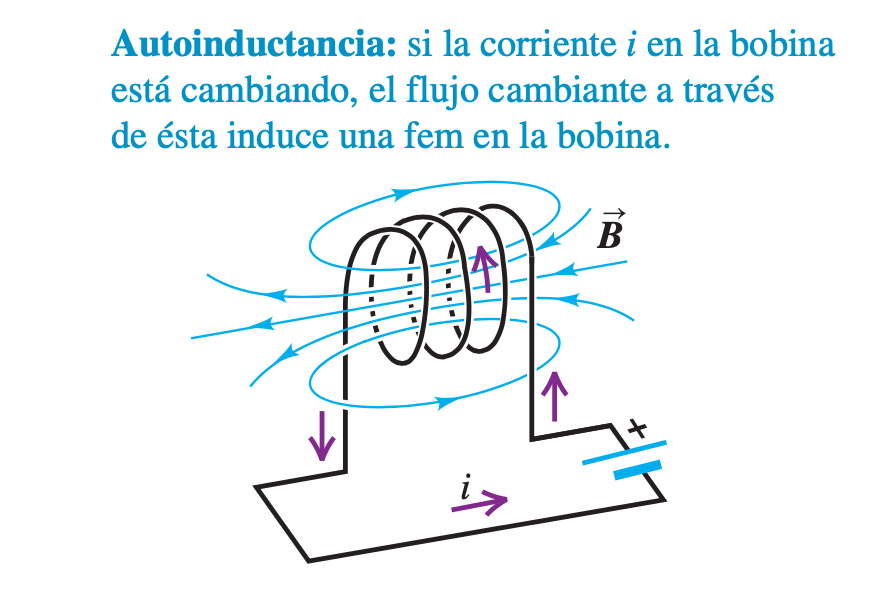
\includegraphics[scale=0.4]{fig/autoinductancia}
\caption{La corriente $i$ en el circuito crea un campo magnético $\vec{B}$ en la bobina y, por lo tanto, un flujo a través de ésta.}
\label{fig:autoinductancia}
\end{figure}

Consideremos un solo circuito aislado. Cuando en el circuito está presente una corriente, se establece un campo magnético que crea un flujo magnético a través del mismo circuito; este flujo cambia cuando la corriente cambia. Así, cualquier circuito que conduzca una corriente variable tiene una fem inducida en él por la variación en su propio campo magnético. Esa clase de fem se denomina \textbf{fem autoinducida}. Según la ley de Lenz, una fem autoinducida siempre se opone al cambio en la corriente que causó la fem, y de ese modo hace más difícil que haya variaciones en la corriente. El efecto se intensifica considerablemente si el circuito incluye una bobina con $N$ espiras de alambre. Como resultado de la corriente $i$, hay un flujo magnético medio $\Phi_B$ a través de cada vuelta de la bobina, figura \ref{fig:autoinductancia}.

Definimos la \textbf{autoinductancia} como
\begin{equation}\label{30.6.autoinductancia}\marginnote{Autoinductancia}
\boxed{L=\frac{N\Phi_B}{i}}
\end{equation}
Si la corriente $i$ en el circuito cambia, también lo hace el flujo $\Phi_B$. De ecuación \ref{30.6.autoinductancia} $$N\frac{d\Phi_B}{dt}=L\frac{di}{dt}$$ Utilizando la ley de Faraday, (\ref{29.4.Nfaraday}), la fem autoinducida es
\begin{equation}\label{30.7}\marginnote{Fem autoinducida}
\boxed{\varepsilon=-L\frac{di}{dt}}
\end{equation}

\subsection{Los inductores como elementos de un circuito}
Un elemento de circuito diseñado para tener una inductancia particular se llama \textbf{inductor, o bobina de autoinducción}. Su finalidad es oponerse a cualquier variación en la corriente a través del circuito. Un inductor en un circuito de corriente directa ayuda a mantener una corriente estable a pesar de las fluctuaciones en la fem aplicada; en un circuito de corriente alterna, un inductor tiende a suprimir las variaciones de la corriente que ocurran más rápido de lo deseado.

Al utilizar la ley de Kirchhoff a traves de una malla conductora se suman sus diferencias de potencial y se igualan a cero porque el campo eléctrico producido por las cargas distribuidas es \textit{conservativo} ($\vec{E_c}$). El campo eléctrico inducido magnéticamente dentro de las bobinas del inductor \textbf{no es conservativo} ($\vec{E_n}$).


\begin{figure}[h]
\centering
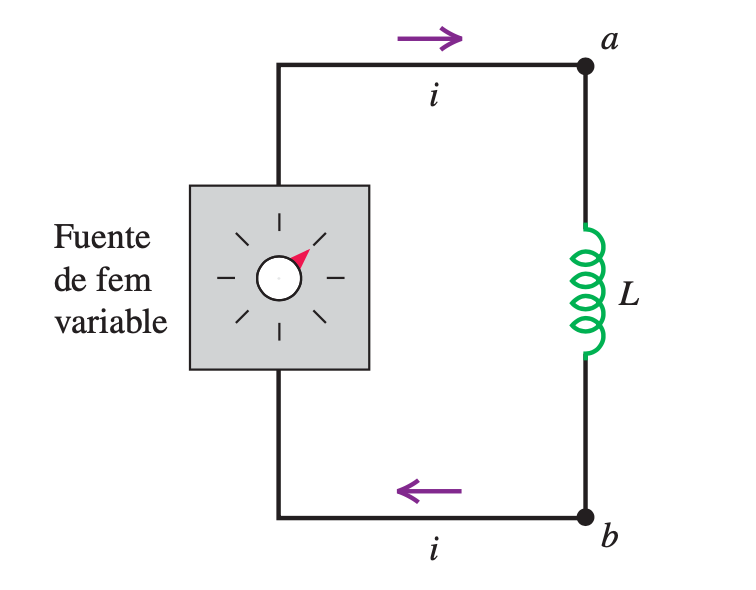
\includegraphics[scale=0.4]{fig/circuito}
\caption{Circuito que contiene una fuente de fem y un inductor. La fuente es variable, por lo que la corriente $i$ y su tasa de cambio $di>dt$ pueden variarse.}
\label{fig30.5.circuito}
\end{figure}

Consideremos el circuito de la figura \ref{fig30.5.circuito}. De acuerdo con la ley de Faraday, (\ref{29.10}), la integral de línea de $\vec{E_n}$ alrededor del circuito es el negativo de la tasa de cambio del flujo a través del circuito. De (\ref{30.7}) $$\oint\vec{E_n}\cdot d\vec{l}=-L\frac{di}{dt}$$ donde se integra en sentido horario del circuito (el sentido supuesto para la corriente). Pero $\vec{E_n}$ es diferente de cero sólo dentro del inductor. Entonces $$\int_a^b\vec{E_n}\cdot d\vec{l}=-L\frac{di}{dt}$$ A continuación, como $\vec{E_c}+\vec{E_n}=0$ en cada punto dentro de las bobinas del inductor $$\int_a^b\vec{E_c}\cdot d\vec{l}=L\frac{di}{dt}$$ Pero esta integral es el potencial $V_{ab}$ del punto $a$ con respecto a $b$

\begin{equation}\label{30.8}
V_{ab}=V_a-V_b=L\frac{di}{dt}
\end{equation}

Se concluye que hay una diferencia de potencial genuina entre las terminales del inductor, asociada con las fuerzas conservativas electrostáticas, a pesar del hecho de que el campo eléctrico asociado con el efecto de inducción magnética es no conservativo.
\textbf{Obervación}: La fem autoinducida se opone a los cambios de la corriente ($di/dt$), \textit{no} a la corriente $i$ en sí.

\section{Energía del campo magnético}
El establecimiento de una corriente en un inductor requiere un suministro de energía, y un inductor que conduce corriente contiene energía almacenada. En la figura \ref{fig30.5.circuito}, una \textit{corriente creciente} $i$ ($di/dt>0$) en el inductor produce una fem $\varepsilon$ entre sus terminales, y una diferencia de potencial correspondiente $V_{ab}$ entre las terminales de la fuente, con el punto $a$ a mayor potencial que el $b$. Así, la fuente debe estar agregando energía al inductor, y la potencia instantánea $P$ (la tasa de transferencia de energía al inductor) es $P=V_{ab}i$.

\subsection{Energía almacenada en un inductor}
Si la corriente inicial es igual a cero, con la inductancia $L$ podemos calcular la entrada total de energía $U$ necesaria para establecer una corriente final $I$ en un inductor. Suponemos que el inductor tiene una resistencia igual a cero, por lo que dentro del inductor no se disipa energía. El voltaje entre las terminales $a$ y $b$ del inductor en ese instante es $V_{ab}=L\frac{di}{dt}$, y la tasa $P$ a la que se entrega energía al indutor (igual a la potencia instantánea suministrada por la fuente) es

\begin{equation*}
P=V_{ab}i=Li\frac{di}{dt}
\end{equation*}

La energía $dU$ suministrada al inductor durante un intervalo de tiempo infinitesimal $dt$ es $dU=Pdt$, por lo que

\begin{equation*}
dU=Lidi
\end{equation*}

La energía total $U$ suministrada mientras la corriente aumenta de cero a un valor final
$I$ es

\begin{equation}\label{30.9}\marginnote{Energía almacenada en un inductor}
\boxed{U=L\int_0^{I}i\, dt=\frac{1}{2}LI^2}
\end{equation}

Una vez que la corriente ha alcanzado su valor final estable $I$, $di/dt=0$, y no se alimenta más energía al inductor. Cuando no hay corriente, la energía almacenada $U$ es igual a cero; cuando la corriente es $I$, la energía es $\frac{1}{2}LI^2$.

Cuando la corriente disminuye de $I$ a cero, el inductor actúa como fuente que suministra una cantidad total de energía igual a $\frac{1}{2}LI^2$ al circuito externo. Si interrumpimos bruscamente el circuito abriendo un interruptor o desconectando violentamente una clavija (enchufe) de una toma de corriente de pared, la corriente disminuye con mucha rapidez, la fem inducida es muy grande y la energía podría disiparse en forma de un arco entre los contactos del interruptor.

\textbf{Observación:} Es importante no confundir el comportamiento de resistores e inductores en lo que respecta a la energía. La energía fluye hacia un resistor siempre que una corriente, ya sea estable o variable, pasa a través de él; esta energía se disipa en forma de calor. En contraste, la energía fluye hacia un inductor ideal con resistencia igual a cero, sólo cuando la corriente en este último se \textit{incrementa}. Esta energía no se disipa, sino que se almacena en el inductor y se libera cuando la corriente \textit{disminuye}. Cuando una corriente estable fluye a través de un inductor, no entra ni sale energía

\subsection{Densidad de la energía magnética}
La energía en un inductor en realidad se almacena en el campo magnético dentro de la bobina, al igual que la energía de un capacitor lo hace en el campo eléctrico entre sus placas. Nos centraremos en un caso sencillo: el del solenoide toroidal ideal. Su campo magnético se encuentra confinado por completo en una región finita del espacio en el interior de su núcleo. La inductancia del selenoide toroidal con vacío dentro de sus bobinas es 

\begin{equation}\label{L de un toroide}\marginnote{Inductancia de un toroide}
L=\frac{\mu_0N^2A}{2\pi r}
\end{equation}

De (\ref{30.9}), la energía $U$ alamacenada en el toroide  cuando la corriente es $I$ es

\begin{equation*}
U=\frac{1}{2}LI^2=\frac{1}{2}\frac{\mu_0N^2A}{2\pi r}I^2
\end{equation*}

El campo magnético y, por lo tanto, esta energía se localizan en el volumen $V=2\pi rA$ encerrado por los devanados. La energía por \textit{unidad de volumen}, o \textit{densidad de energía magnética}, es $u=U/V$:

\begin{equation}\label{u}
u=\frac{U}{2\pi rA}=\frac{1}{2}\mu_0\frac{N^2I^2}{(2\pi r)^2}
\end{equation}

Expresandola en términos de la magnitud $B=(\mu_0NI)/(2\pi r)$ del campo magnético dentro del toroide es

\begin{equation*}
\frac{N^2I^2}{(2\pi r)^2}=\frac{B^2}{\mu_0^2}
\end{equation*}

Sustituyendo esto en (\ref{u}), se encuentra que la expresión para la \textbf{densidad de energía magnética} en el vacío es

\begin{equation}\label{30.10.u}\marginnote{Densidad de energía magnética en el vacío}
\boxed{u=\frac{B^2}{2\mu_0}}
\end{equation}

Cuando el material dentro del toroide no es un vacío, sino un material con permeabilidad magnética (constante) $\mu=K_m\mu_0$, se sustituye $\mu_0$ por $\mu_0$ en (\ref{30.10.u}). Así, la energía por unidad de volúmen en el campo magnético es

\begin{equation}\label{30.11.u2}\marginnote{Densidad de energía magnética en un material}
\boxed{u=\frac{B^2}{2\mu}}
\end{equation}

La expresión \ref{30.11.u2} resulta ser correcta para \textit{cualquier} configuración de campo magnético en un material con permeabilidad constante. 

\section{El circuito R-L}
Un inductor en un circuito hace difícil que ocurran cambios rápidos en la corriente, en virtud de los efectos de la fem autoinducida. La ecuación \ref{30.7} muestra que cuanto más grande es la tasa de cambio de la corriente, $di/dt$, mayor es la fem autoinducida y mayor la diferencia de potencial entre las terminales del inductor.

\subsection{Crecimiento de la corriente en un circuito R-L}

\begin{figure}[h]
\centering
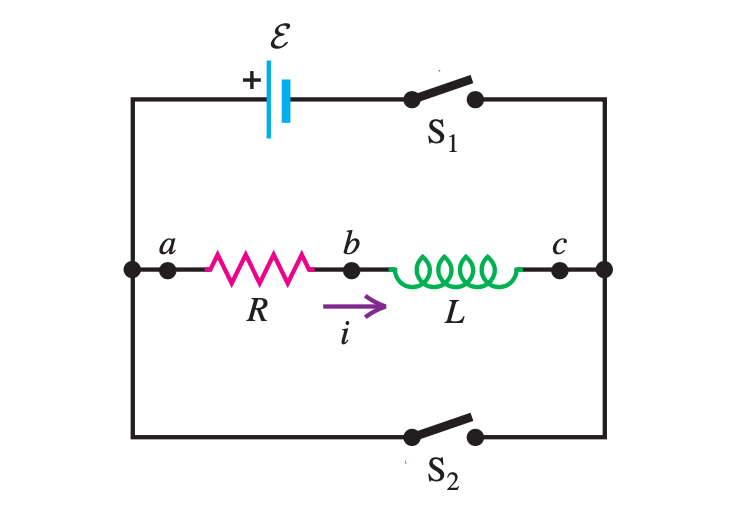
\includegraphics[scale=0.4]{fig/circuito2}
\caption{Al cerrar el interruptor $S_1$ se conecta la combinación $R-L $en serie con una fuente de fem $\varepsilon$. Al cerrar el interruptor $S_2$ al mismo tiempo que se abre $S_1$ se desconecta la combinación de la fuente.}
\label{fig:circuito2}
\end{figure}

Un circuito que incluye tanto un resistor como un inductor, y tal vez una fuente de fem, se llama circuito R-L (figura \ref{fig:circuito2}).  El inductor ayuda a impedir los cambios rápidos en una corriente, lo que puede ser útil si se requiere una corriente estable y la fuente externa tiene una fem fluctuante. Al cerrar el interruptor $S_1$ se conecta la combinación R-L a una fuente con fem constante $\varepsilon$. 

Suponga que, en un principio, ambos interruptores están abiertos, y luego, en cierto momento inicial $t=0$ se cierra el interruptor $S_1$. La corriente no puede cambiar súbitamente de cero a algún valor final porque $di/dt$ y la fem inducida en el inductor serían infinitas. En vez de ello, la corriente comienza a crecer con una tasa que sólo depende del valor de $L$ en el circuito.

Sea $i$ la corriente en cierto momento $t$ después de que se cerró el interruptor $S_1$, y sea $di/dt$ su tasa de cambio en ese instante. La diferencia de potencial $v_{ab}$ a través del resistor en ese momento es

\begin{equation*}
v_{ab}=iR
\end{equation*}

y la diferencia de potencial $v_{bc}$ a través del inductor es

\begin{equation*}
v_{bc}=L\frac{di}{dt}
\end{equation*}

Aplicamos la ley de mallas de Kirchhoff, comenzando en la terminal negativa y avanzando en sentido antihorario alrededor del circuito:

\begin{equation}\label{30.12}
\varepsilon - iR - L\frac{di}{dt}=0
\end{equation}
\begin{equation}\label{30.13}
\frac{di}{dt}=\frac{\varepsilon -iR}{L}=\frac{\varepsilon}{L}-\frac{R}{L}i
\end{equation}
 En el instante en que el interruptor $S_1$ se cierra por primera vez, $i = 0$ y la caída del potencial a través de $R$ es igual a cero. La tasa de cambio inicial de la corriente es
 
\begin{equation*}
\left(\frac{di}{dt}\right)_{inicial}=\frac{\varepsilon}{L}
\end{equation*}
 Como se esperaba, cuanto mayor es la inductancia $L$, con más lentitud aumenta la corriente.
 
Conforme aumenta la corriente, el término $(R/L)i$ en (\ref{30.13}) también aumenta, y la tasa de incremento de la corriente dada por (\ref{30.13}) se hace cada vez más pequeña. Esto significa que la corriente se acerca a un valor final $I$ de estado estable. Cuando la corriente alcanza ese valor, su tasa de incremento es igual a cero. Entonces, la ecuación \ref{30.13} se convierte en:

\begin{align*}
\left(\frac{di}{dt}\right)_{final}&=0=\frac{\varepsilon}{L}-\frac{R}{L}i \\
\Rightarrow  I&=\frac{\varepsilon}{R}
\end{align*}

La corriente \textit{final} $I$ no depende de la inductancia $L$; es la misma que se tendría si sólo se conectara la resistencia $R$ a la fuente con fem $\varepsilon$.

Para obtener el comportamiento de la corriente en función del tiempo, se reordena (\ref{30.13}):

\begin{equation*}
\frac{di}{i-(\varepsilon /R)}=-\frac{R}{L}dt
\end{equation*}

Cambiando el nombre de las variables de integración a $i'$ y $t'$ para utilizar $i$ y $t$ como límites superiores

\begin{align*}
\int_0^{i}\frac{di'}{i'-(\varepsilon /R)}&=-\int_0^{t}\frac{R}{L}dt' \\
\ln\left(\frac{i-(\varepsilon /R)}{-\varepsilon /R}\right)&=-\frac{R}{L}t
\end{align*}

Despejando la corriente $i$

\begin{equation}\label{30.14}\marginnote{Corriente en un circuito R-L con fem}
\boxed{i=\frac{\varepsilon}{R}(1-e^{-(R/L)t})}
\end{equation}

(\ref{30.14}) se obtiene

\begin{equation}\label{30.15}
\frac{di}{dt}=\frac{\varepsilon}{L}e^{-(R/L)t}
\end{equation}

En el momento $t=0$, $i=0$ y $di/dt=\varepsilon /L$. Conforme $t\to\infty$, $i\to \varepsilon /R$ y $di/dt\to 0$, como se había pronosticado. Este comportamiento se ve representado en la figura \ref{fig:rl-grafico}

\begin{figure}[h]
\centering
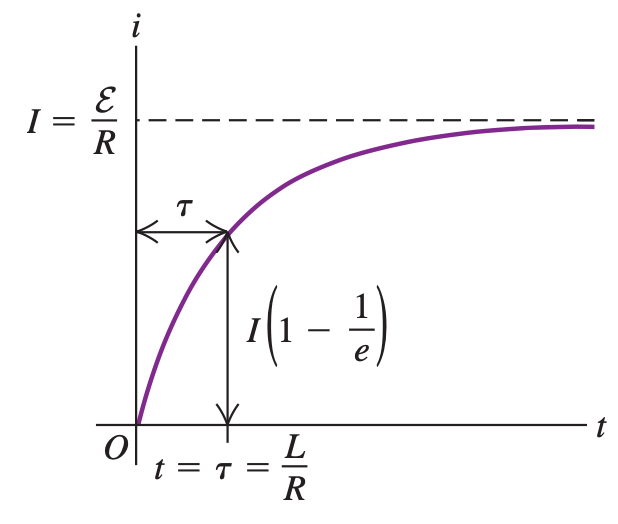
\includegraphics[scale=0.5]{fig/rl-grafico}
\caption{Curva de la ecuación \ref{30.14}}
\label{fig:rl-grafico}
\end{figure}

En un tiempo igual a $L/R$ la corriente ha subido a $(1-1/e)$, o el $63\%$ de su valor final. De esta forma, la cantidad $L/R$ es una medida de la rapidez con que la corriente se aproxima a su valor final; esta cantidad se llama \textit{constante de tiempo} del circuito, y se denota con $\tau$:

\begin{equation}\label{30.16}\marginnote{Constante de tiempo para un circuito R-L}
\tau=\frac{L}{R}
\end{equation}

Las consideraciones acerca de la energía brindan una perspectiva adicional sobre el comportamiento de un circuito R-L. La tasa instantánea con la que la fuente entrega energía al circuito es $P=\varepsilon i$. La tasa instantánea con que se disipa energía en el resistor es $i^2R$, y la tasa con que se almacena energía en el inductor es $iv_{bc}=Li\, di/dt$ [o, en forma equivalente, $(d/dt)(\frac{1}{2}Li^2)=Li\, di/dt$]. Multiplicando (\ref{30.12}) y reordenando se obtiene

\begin{equation}\label{30.17}
\varepsilon i=i^2R+Li\frac{di}{dt}
\end{equation}

De la potencia $\varepsilon i$ suministrada por la fuente, la parte $(i^2R)$ se disipa en el resistor, y la parte $(Li\, di/dt)$ es la energía almacenada en el inductor.

\subsection{Decaimiento de la corriente en un circuito R-L}
Ahora supongamos que el interruptor $S_1$ en el circuito de la figura \ref{fig:circuito2} ha permanecido cerrado por un tiempo y la corriente ha alcanzado el valor $I_0$. Se reinicia el cronómetro para redefinir el tiempo inicial, se cierra el interruptor $S_2$ en el momento $t=0$, con la batería puesta en derivación. La ecuación de la ley de Kirchhoff de las mallas se obtiene (\ref{30.12}), con sólo omitir el término $\varepsilon$. Haciendo los cálculos se ecuentra que la corriente varía con el tiempo de acuerdo con

\begin{equation}\label{30.18}
\boxed{i=I_0e^{-(R/L)t}}
\end{equation}

donde $I_0$ es la corriente inicial en el momento $t=0$

\begin{figure}[h]
\centering
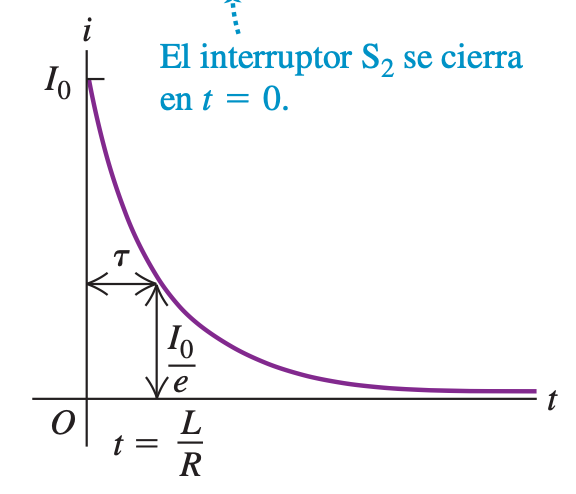
\includegraphics[scale=0.4]{fig/r-l-desconexion}
\caption{Curva de la ecuación \ref{30.18}}
\label{fig:r-l-desconexion}
\end{figure}

La energía necesaria para mantener la corriente durante este decaimiento proviene de la energía almacenada en el campo magnético del inductor. En vez de (\ref{30.17}) tenemos

\begin{equation}\label{30.19}
0=i^2R+Li\, \frac{di}{dt}
\end{equation}

\section{El circuito L-C}
Un circuito que contiene un inductor y un capacitor muestra un modo completamente nuevo de comportamiento, caracterizado por una corriente y una carga \textit{oscilantes}.

\begin{figure}[h]
\centering
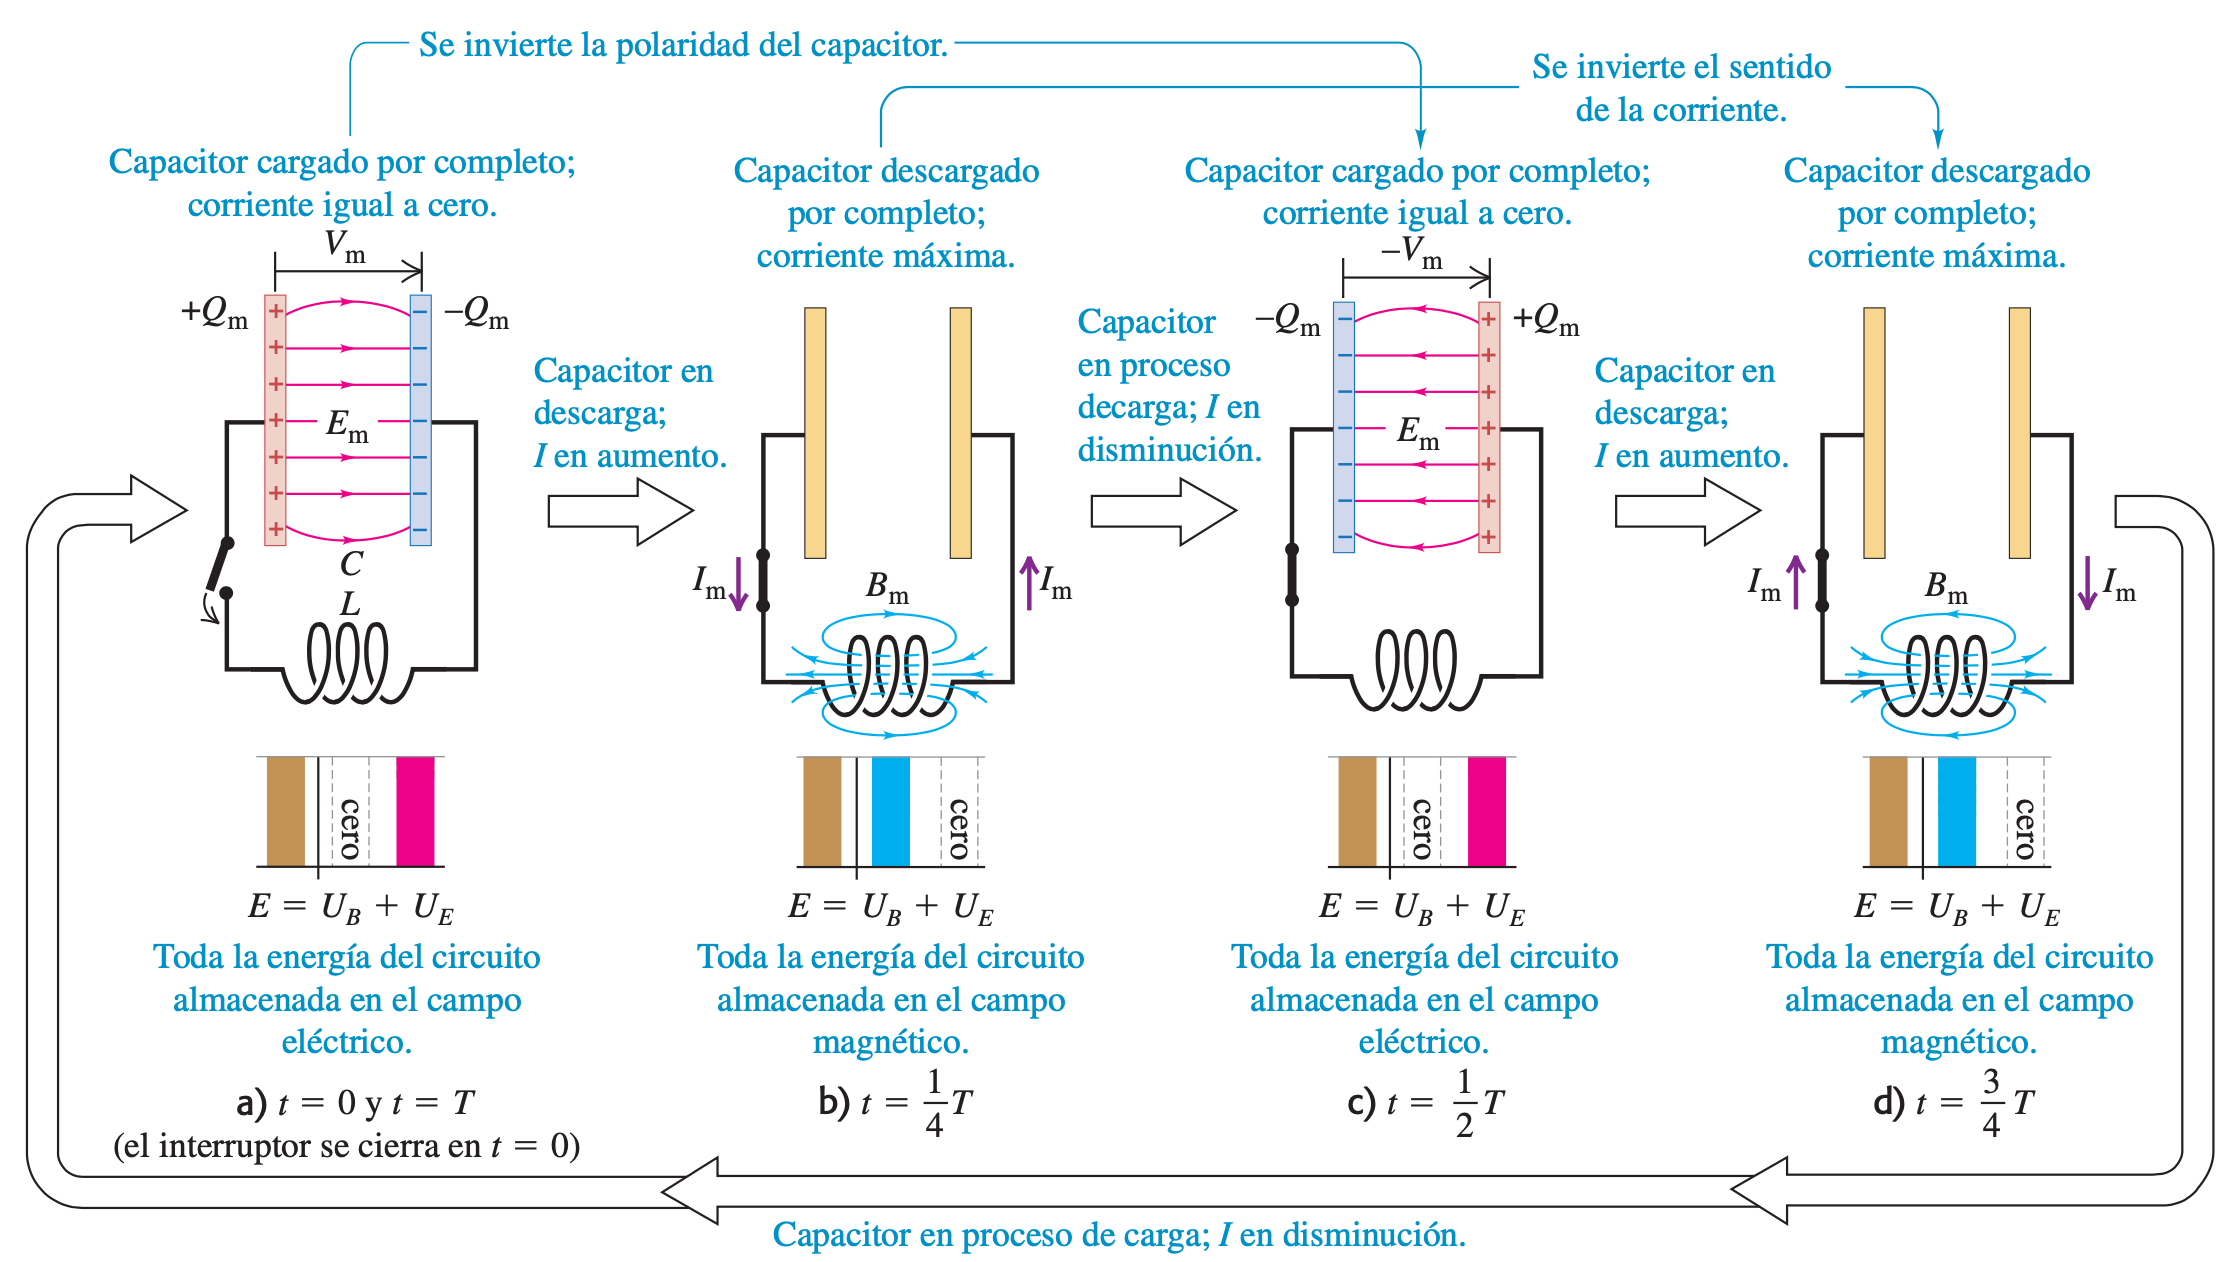
\includegraphics[scale=0.4]{fig/circuito-l-c}
\caption{En un circuito oscilante L-C, la carga en el capacitor y la corriente a través del inductor varían en forma sinusoidal con el tiempo. Se transfiere energía entre la energía magnética en el inductor $(U_B)$ y la energía eléctrica en el capacitor $(U_E)$. Como en el movimiento armónico simple, la energía total $E$ permanece constante.}
\label{fig:circuito-l-c}
\end{figure}

En el \textbf{circuito L-C} de la figura \ref{fig:circuito-l-c} se carga el capacitor con una diferencia de potencial $V_m$ y una carga inicial $Q=CV_m$ en su placa izquierda y luego se cierra el interruptor. El capacitor comienza a descargar a través del inductor. A causa de la fem inducida en el inductor, la corriente no puede cambiar en forma instantánea; comienza en cero y finalmente alcanza un valor máximo $I_m$. Durante esta intensificación el capacitor se está descargando. En cada instante el potencial del capacitor es igual a la fem inducida, por lo que a medida que el capacitor se descarga, la tasa de cambio de la corriente disminuye. Cuando el potencial del capacitor se reduce a cero, la fem inducida también es igual a cero, y la corriente se ha estabilizado en su valor máximo $I_m$. Durante la descarga del capacitor, la corriente en aumento en el inductor ha establecido un campo magnético en el espacio que lo rodea, y la energía que inicialmente estaba almacenada en el campo eléctrico del capacitor ahora lo está en el campo magnético del inductor. La corriente persiste (no puede cambiar instantáneamente), y el capacitor comienza a cargarse con polaridad opuesta a la de su estado inicial. Conforme disminuye la corriente, la magnitud del campo magnético también lo hace, lo que induce una fem en el inductor en el mismo sentido que el de la corriente; esto retarda la disminución de la corriente. Con el tiempo, la corriente y el campo magnético disminuyen a cero y el capacitor queda cargado en el sentido opuesto al de su polaridad inicial, con una diferencia de potencial $-V_m$ y carga $-Q$ en su placa izquierda. El proceso se repite ahora en sentido opuesto; un poco después, el capacitor se ha descargado una vez más y en el inductor hay una corriente en el sentido opuesto . Más tarde, la carga del capacitor recupera su valor original, y todo el proceso se repite. Si no hay pérdidas de energía, las cargas en el capacitor siguen oscilando hacia atrás y adelante indefinidamente. Este proceso se llama \textbf{oscilación eléctrica}. Desde el punto de vista de la energía, las oscilaciones de un circuito eléctrico transfieren energía del campo eléctrico del capacitor al campo magnético del inductor y viceversa. La energía \textit{total} asociada con el circuito es constante. Esto es análogo a la transferencia de energía en un sistema mecánico que oscila de la energía potencial a la cinética y viceversa, con la energía total constante.

\subsection{Oscilaciones eléctricas en un circuito L-C}
Según la ley de Kirchhoff de las mallas

\begin{equation*}
-L\frac{di}{dt}-\frac{q}{C}=0
\end{equation*}

Aplicando $i=dq/dt$ y reordenando

\begin{equation}\label{30.20}\marginnote{Circuito L-C}
\frac{d^2q}{dt^2}+\frac{1}{LC}q=0
\end{equation}

La ecuación \ref{30.20} tiene la misma forma de la expresión que se obtuvo para el movimiento armónico simple

\begin{equation*}
\frac{d^2x}{dt^2}+\frac{k}{m}x=0
\end{equation*}

En el circuito L-C la carga del capacitor q desempeña el papel del desplazamiento $x$, y la corriente $i=dq/dt$ es análoga a la velocidad de la partícula $v_x=dx/dt$. La inductancia $L$ es análoga a la masa $m$, y el recíproco de la capacitancia, $1/C$, es análogo a la constante de fuerza $k$.

Continuando con esta analogía, recordamos que la frecuencia angular $\omega=2\pi f$ del oscilador armónico es igual a $\sqrt{k/m}$, y la posición está dada en función del tiempo por

\begin{equation*}
x=A\cos (\omega t + \phi)
\end{equation*}

donde la amplitud $A$ y el ángulo de fase $\phi$ dependen de las condiciones iniciales.

En la situaación eléctrica se tiene

\begin{equation}\label{30.21}
q=Q\cos (\omega t +\phi)
\end{equation}

y la frecuencia angular v de la oscilación está dada por

\begin{equation}\label{30.22}
\omega=\sqrt{\frac{1}{LC}}
\end{equation}

Luego, la corriente instantánea $i=dq/dt$ está dada por

\begin{equation}\label{30.23}
i=-\omega Q\sin (\omega t + \phi)
\end{equation}

Así, en un circuito L-C la carga y la corriente oscilan en forma sinusoidal con el tiempo, con una frecuencia angular determinada por los valores de $L$ y $C$. La frecuencia ordinaria $f$, el número de ciclos por segundo, es igual a $v/2\pi$, como siempre. En (\ref{30.21}) y (\ref{30.23}), las constantes $Q$ y $\phi$ están determinadas por las condiciones iniciales.

\subsubsection{Energía en un circuito L-C}
En el problema mecánico, un cuerpo con masa $m$ está sujeto a un resorte con constante de fuerza $k$. Suponga que el cuerpo se desplaza una distancia $A$ desde su posición de equilibrio y se le libera desde el reposo en el tiempo $t=0$. La energía cinética del sistema en un isntante posterior es 	$\frac{1}{2}mv_x^2$, y su energía potencial elástica es $\frac{1}{2}kx^2$. Como el sistema es conservativo, la suma de estas energías es igual a la energía inicial del sistema, $\frac{1}{2}kA^2$. La velocidad $v_x$ en cualquier posición está dada por

\begin{equation}\label{30.24}
v_x=\pm\sqrt{\frac{k}{m}}\sqrt{A^2-x^2}
\end{equation}

El circuito L-C también es un sistema conservativo. Otra vez, sea $Q$ la carga máxima del capacitor. La energía del campo magnético, $\frac{1}{2}Li^2$, en el inductor en cualquier momento corresponde a la energía cinética $\frac{1}{2}mv^2$ del cuerpo oscilante, y la energía del campo eléctrico $q^2/2C$ en el capacitor corresponde a la energía potencial elástica $\frac{1}{2}kx^2$ del resorte. La suma de estas energías es igual a la energía total $Q^2/2C$ del sistema:

\begin{equation}\label{30.25}
\frac{1}{2}Li^2+\frac{q^2}{2C}=\frac{Q^2}{2C}
\end{equation}

La energía total en el circuito L-C es \textit{constante}; oscila entre las formas magnética y eléctrica.

Despejando $i$ de (\ref{30.25}) se encuentra que cuando la carga en el capacitor es $q$, la corriente $i$ es

\begin{equation}\label{30.26}
i=\pm\sqrt{\frac{1}{LC}}\sqrt{Q^2-q^2}
\end{equation}

\section{El circuito L-R-C en serie}
La resistencia en un circuito eléctrico es análoga a la fricción en un sistema mecánico. Suponga que un inductor con inductancia $L$ y un resistor de resistencia $R$ están conectados en serie entre las terminales de un capacitor cargado, para formar un \textbf{circuito en serie $L-R-C$}. Como antes, el capacitor comienza a descargarse tan pronto como el circuito está completo.

Si la resistencia $R$ es relativamente pequeña, el circuito aún oscila, pero con un \textbf{movimiento armónico amortiguado}, y se dice que el circuito está \textbf{subamortiguado}. Si $R$ se incrementa, las oscilaciones cesan con más rapidez. Cuando $R$ alcanza cierto valor, el circuito deja de oscilar; está \textbf{críticamente amortiguado}. Para valores aún mayores de $R$, el circuito está \textbf{sobreamortiguado}, y la carga del capacitor se acerca a cero aún más lentamente.

\subsection{Análisis del circuito $L-R-C$}
Primero se cierra el interruptor en la posición hacia arriba, para conectar al capacitor con una fuente de fem $\varepsilon$ durante un tiempo suficientemente largo para asegurar que el capacitor adquiera su carga final $Q=C\varepsilon$ y que toda oscilación inicial haya cesado. Entonces, en el momento $t=0$ se coloca al interruptor en la posición hacia abajo, con lo que se elimina a la fuente del circuito y se pone al capacitor en serie con el resistor y el inductor. Aplicando Kirchoff:

\begin{equation*}
-iR-L\frac{di}{dt}-\frac{q}{C}=0
\end{equation*}

\begin{equation}\label{30.27}
\frac{d^2q}{dt^2}+\frac{R}{L}\frac{dq}{dt}+\frac{1}{LC}q=0
\end{equation}

Hay métodos generales para obtener soluciones (\ref{30.27}). La forma de la solución es diferente para los casos del circuito subamortiguado ($R$ pequeña) y sobreamortiguado ($R$ grande). Cuando $R^2$ es menor que $4L/C$, la solución tiene la forma

\begin{equation}\label{30.28}
q=Ae^{-(R/2L)t}\cos \left(\sqrt{\frac{1}{LC}-\frac{R^2}{4L^2}t}+\phi\right)
\end{equation}

donde $A$ y $\phi$ son constantes.

Esta solución corresponde al comportamiento \textit{subamortiguado}; la función representa una oscilación sinusoidal con una amplitud que decae exponencialmente. Notar que

\begin{equation}\label{30.29}\marginnote{Circuito en serie $R-C-L$ subamortiguado}
\boxed{\omega '=\sqrt{\frac{1}{LC}-\frac{R^2}{4L^2}}}
\end{equation}

















































